\documentclass[11pt]{amsart}
\usepackage[margin=1.05in]{geometry}
\usepackage{amsmath,amssymb,amsthm}
\usepackage{booktabs}
\usepackage{array}
\usepackage{enumitem}
\usepackage{pgfplots}
\pgfplotsset{compat=1.16}
\usepackage[hidelinks]{hyperref}

\newtheorem{theorem}{Theorem}[section]
\newtheorem{lemma}[theorem]{Lemma}
\newtheorem{proposition}[theorem]{Proposition}
\newtheorem{corollary}[theorem]{Corollary}
\newtheorem{conjecture}[theorem]{Conjecture}
\newtheorem*{theoremA}{Theorem A}
\newtheorem*{theoremB}{Theorem B}
\newtheorem*{theoremC}{Theorem C}
\newtheorem*{theoremD}{Theorem D}
\newtheorem*{tuzconj}{Conjecture 3.7 of \cite{TUZ}}
\theoremstyle{definition}
\newtheorem{definition}[theorem]{Definition}
\newtheorem{problem}{Problem}
\renewcommand{\theproblem}{\Alph{problem}}
\theoremstyle{remark}
\newtheorem{remark}[theorem]{Remark}
\newtheorem{example}[theorem]{Example}

\newcommand{\Z}{\mathbb{Z}}
\newcommand{\N}{\mathbb{N}}
\newcommand{\cen}{\mathcal{C}}

\title[Tent rigidity for the Erd\H{o}s--Graham equation]{Tent rigidity for the Erd\H{o}s--Graham equation $\frac{n}{2^n}=\sum_{i=1}^k\frac{a_i}{2^{a_i}}$\\ and the Tengely--Ulas--Zygad\l{}o conjecture}
\author{Keio}
\date{October 29, 2026}

\begin{document}

\begin{abstract}
For a dyadic rational $x$ we study the set of all representations $x=\sum_{a\in A}a2^{-a}$ with $A$ a set of positive integers. Writing the remainder after step $j$ as an integer state $\rho_j$ and measuring its signed offset $v_j=2\rho_j-j-2$ from the centre of the admissible interval, we prove a rigidity theorem: along \emph{every} path whose states stay strictly inside the interval, $|v_j|$ is the $j$-th term of one and the same integer sequence
$u_{j+1}=|2u_j-(j+1)|$.
Consequently every representation is obtained by independent binary choices at the zeros of $(u_j)$, possibly followed by a stop at a time where $u_j=1$; after the starting time these zeros occur only at $j\equiv 2\pmod 4$. Finite representations end exactly where $u_j=1$ on the lower side; representations of $n/2^n$ with largest term $K$ exist only if $u_{K-1}=1$, and then they are $2^{h-1}$ in number when $h\ge1$ zeros precede $K-1$; and their numbers of terms form an explicit subset-sum set.

We apply this to the equation $n/2^n=\sum_{i=1}^k a_i/2^{a_i}$ of Erd\H{o}s and Graham (Erd\H{o}s Problem \#261). (i) The inequality $a_k\le 2(k+n)$ of Conjecture~3.7 of Tengely, Ulas and Zygad\l{}o (J.~Number Theory 2020) is false: $n=3$, $k=185$, $a_k=392$ is a counterexample. Among all solutions, $392$ is the least largest term and $177$ the least number of terms of a counterexample, and for $n=3$ the excess $a_k-2(n+k)$ reaches $21300$ below $2\cdot10^9$; on the other hand the inequality holds whenever $n\ge k(1+\log_2k+\log_2\log_2 4k)$, previously known for $n\ge 2^k-k$. (ii) The consequence $a_k\le 4(2^k-1)$ stated in the same conjecture is true: every solution satisfies $a_k\le 2^{k+1}-2$, with equality only for $n=2^{k+1}-k-2$, $a_i=n+i$. This bound is optimal. (iii) We determine all solutions with at most $28$ terms (listed in the supplementary archive), correcting the published list for $k=8$. (iv) We reformulate two parts of Problem \#261 in terms of $(u_j)$ and verify that $n/2^n$ is representable for every $n\le 10^6$. We also observe that a counterexample to (i) can be read off from a 1990 table of Borwein and Loring.
\end{abstract}

\maketitle

\section{Introduction}

Let $f(a)=a\,2^{-a}$. Erd\H{o}s and Graham \cite{EG80} asked about the equation
\begin{equation}\label{eq:EG}
\frac{n}{2^n}=\sum_{i=1}^{k}\frac{a_i}{2^{a_i}},\qquad k\ge 2,\quad 1\le a_1<a_2<\dots<a_k ,
\end{equation}
in positive integers. In the formulation of Erd\H{o}s Problem \#261 \cite{EP261} the questions are: are there infinitely many $n$ for which \eqref{eq:EG} is solvable; is it solvable for all $n$; and is there a rational $x$ with at least $2^{\aleph_0}$ representations $x=\sum_{k\ge1}a_k/2^{a_k}$? According to \cite{EP261}, Erd\H{o}s \cite{Er88} attributes a simple proof of the first to Cusick; Borwein and Loring \cite{BL90} observed that $n=2^{m+1}-m-2$ admits the \emph{consecutive} solution $a_i=n+i$ $(1\le i\le m)$, studied a greedy ``base change'' algorithm and conjectured that it always terminates \cite[Conj.~1]{BL90}, which would settle the second question. Tengely, Ulas and Zygad\l{}o \cite{TUZ} verified solvability for $n\le 10^4$, listed all solutions with $k\le 8$, proved
\begin{equation}\label{eq:TUZbound}
a_k\le 2^{k+2}+2k(\log_2k-1)-4\qquad\text{\cite[Cor.~2.9]{TUZ}},
\end{equation}
and, on the basis of greedy solutions for $n\le 5000$, formulated:

\begin{tuzconj}
If $(n,k,a_1,\dots,a_k)$ is a solution of \eqref{eq:EG} with $a_1<\dots<a_k$, then $k+n\le a_k\le 2(k+n)$. In particular $a_k\le 4(2^k-1)$.
\end{tuzconj}

The lower inequality is elementary and sharp \cite[Rem.~3.8]{TUZ}; the upper one was proved there for $n\ge 2^k-k$. The ``in particular'' clause follows from the upper inequality and $n\le 2^{k+1}-k-2$ \cite[Thm.~2.1]{TUZ}.

\subsection*{A new problem and a new method}
All three questions concern the \emph{set} of representations of a fixed dyadic rational, so we first pose the following structural problem.

\begin{problem}[the window problem]\label{prob:A}
Let $x>0$ be dyadic and let $N\ge0$ with $2^Nx\in\Z$. Describe the set of all $A\subseteq\Z_{>N}$ with $\sum_{a\in A}f(a)=x$: for which $K$ is there a finite such $A$ with $\max A=K$, how many are there, which cardinalities $|A|$ occur, and when is the set uncountable?
\end{problem}

The remainder $\rho_j=2^j\sum_{a\in A,\,a>j}f(a)$ is an integer in $[0,j+2]$ and evolves by $\rho_{j+1}=2\rho_j$ or $2\rho_j-(j+1)$ (Section~\ref{sec:states}). The key observation is that the offset $v_j=2\rho_j-(j+2)$ from the centre of $[0,j+2]$ has an absolute value that does not depend on the choices made.

\begin{theoremA}[tent rigidity; Theorems \ref{thm:rigid}, \ref{thm:count}, \ref{thm:blocks}]
Let $u_N=|2\rho_N-N-2|$ and $u_{j+1}=|2u_j-(j+1)|$. Every admissible path with live states satisfies $|v_j|=u_j$. Live paths branch exactly at the \emph{centres} $u_j=0$ (which satisfy $j\equiv2\pmod4$ when $j>N$); a finite representation with largest term $K$ exists only if $u_{K-1}=1$, and then their number is $2^{h-1}$ if $h\ge1$ centres lie in $[N,K-1)$. After the first centre the set of live states is symmetric under $\rho\mapsto j+2-\rho$, the two choices at each centre produce complementary inclusion patterns up to the next centre, and the cardinalities of the representations with largest term $K$ are exactly the subset sums $1+A_0+y+\sum_{i<h}\xi_i$, $\xi_i\in\{x_i,L_i-x_i\}$, of explicitly computable block data. The set of all representations of $x$ above level $N$ is uncountable if and only if $(u_j)$ has infinitely many zeros.
\end{theoremA}

For $x=n/2^n$ one takes $N=n$, $\rho_n=n$, $u_n=|n-2|$; by Lemma~\ref{lem:a1} every solution of \eqref{eq:EG} has all $a_i>n$, so Theorem~A describes \emph{all} solutions for a given $n$. It reduces the search for solutions with largest term $\le J$ to one pass over a single integer sequence.

\subsection*{Application: Conjecture 3.7 is half false and half true}

\begin{theoremB}[Theorem \ref{thm:counter}]
The upper inequality $a_k\le 2(k+n)$ of Conjecture~3.7 is false: \textup{(a)} the set $A^*$ listed at the beginning of Section~\ref{sec:counter} satisfies $\sum_{a\in A^*}a/2^a=3/8$, $|A^*|=185$, $\max A^*=392>376=2(185+3)$. Moreover \textup{(}the letters refer to Theorem~\ref{thm:counter}\textup{)}:
\begin{enumerate}[label=\textup{(\alph*)},start=2]
\item every solution with $a_k\le 391$ satisfies $a_k\le 2(k+n)$; exactly $37$ of the $403$ solutions with $a_k\le392$ violate it, all with $a_k=392$;
\item every solution with $k\le 176$ satisfies $a_k\le 2(k+n)$, and the only counterexample with $k=177$ is $n=18$, $a_k=392$;
\item for $n=3$ there are counterexamples with $a_k=392$, $12230$, $55328$, $155942$, $460536$, $3254286$, \dots, $753950542$; the excess $a_k-2(n+k)$ is $16$ for $a_k=392$ and $21300$ for $a_k=753950542$;
\item for every $n\le 16513$ there is a counterexample with this $n$.
\end{enumerate}
\end{theoremB}

\begin{theoremC}[Theorem \ref{thm:sharp}]
Every solution of \eqref{eq:EG} satisfies $a_k\le 2^{k+1}-2$, with equality if and only if $n=2^{k+1}-k-2$ and $a_i=n+i$ for $1\le i\le k$. In particular $a_k\le 4(2^k-1)$, so the second sentence of Conjecture~3.7 is true.
\end{theoremC}

Theorem~C is optimal and improves \eqref{eq:TUZbound}; it gives the optimal answer to \cite[Question~1.2]{TUZ} (``Is it possible to bound $a_k$ in terms of $k$ only?''). Its proof combines a gap lemma (Lemma~\ref{lem:gap}) coming from the state formalism with an elementary extremal inequality. The same gap lemma shows that the upper inequality $a_k\le2(k+n)$ does hold whenever $n\ge k(1+\log_2k+\log_2\log_2(4k))$, improving the range $n\ge2^k-k$ of \cite[Rem.~3.8]{TUZ} from exponential to $O(k\log k)$ (Proposition~\ref{prop:region}).

\begin{theoremD}[Section \ref{sec:Nk}]
For $2\le k\le 28$ the number $N(k)$ of solutions of \eqref{eq:EG} with exactly $k$ terms is given in Table~\ref{tab:Nk}. In particular the list of \cite[Thm.~2.5]{TUZ} for $k=8$ misses the solution $n=35$, $(a_i)=(36,37,38,39,42,43,45,46)$.
\end{theoremD}

Theorem~A also turns two parts of Problem \#261 into statements about the single sequence $(u_j)$ (Corollaries \ref{cor:ii} and \ref{cor:iii}); we use this to verify solvability of \eqref{eq:EG} for all $n\le 10^6$ (previously $n\le10^4$ \cite{TUZ}). These parts of Problem \#261 remain open.

\begin{remark}[priority]\label{rem:BL}
Borwein and Loring \cite[\S5]{BL90} tabulated representations of $(m-2)/2^m=f(m-1)-f(m)$ of minimal length. Their row $m=15$ lists a minimal representation with termination term $393$ and $180$ terms, found after $2$ branchings (the greedy one has $186$ terms); by their conversion rule (one more term, largest term one less) it is a solution of \eqref{eq:EG} with $n=14$, $k=181$, $a_k=392>390=2(k+n)$. We recomputed it: it is one of the $37$ solutions in Theorem~B(a), and the two solutions for $n=14$ with $a_k=392$ have $181$ and $187$ terms. Thus a counterexample to the upper inequality was implicitly available thirty years before the conjecture was made. The rigidity statement, the counting formula and the block structure of Theorem~A do not appear in \cite{BL90}, whose Algorithm~3 enumerates representations by branching at window states.
\end{remark}

\subsection*{Organization}
Section~\ref{sec:states} sets up the integer states and proves the gap lemma and an extremal inequality. Section~\ref{sec:tent} proves Theorem~A. Sections~\ref{sec:counter} and \ref{sec:sharp} prove Theorems B and C. Section~\ref{sec:Nk} contains the complete solution counts for $k\le28$, and Section~\ref{sec:261} the consequences for Problem \#261. Section~\ref{sec:cert} describes the computations and how to check them. The counterexample $A^*$ is listed at the beginning of Section~\ref{sec:counter}.

\section{Integer states}\label{sec:states}

\begin{lemma}\label{lem:a1}
If $(n;a_1<\dots<a_k)$ solves \eqref{eq:EG}, then $a_1\ge n+1$.
\end{lemma}

\begin{proof}
We have $f(1)=f(2)=\tfrac12$ and $f(a+1)/f(a)=\frac{a+1}{2a}<1$ for $a\ge2$, so $f$ is non-increasing on $\Z_{\ge1}$ and strictly decreasing on $\Z_{\ge2}$. If $a_1\le n$, then $f(a_1)\ge f(n)$ and $\sum_i f(a_i)\ge f(a_1)+f(a_k)>f(n)$ because $k\ge2$.
\end{proof}

Fix an integer $N\ge0$ and a dyadic $x>0$ with $2^Nx\in\Z$. A \emph{representation of $x$ above level $N$} is a set $A\subseteq\Z_{>N}$, finite or infinite, with $\sum_{a\in A}f(a)=x$. For $A$ such a representation and $j\ge N$ put
\[
\rho_j=\rho_j(A)=2^j\sum_{a\in A,\ a>j}f(a).
\]

\begin{lemma}\label{lem:states}
\begin{enumerate}[label=\textup{(\roman*)}]
\item $\rho_N=2^Nx$ and $\rho_{j+1}=2\rho_j-(j+1)\,[\,j+1\in A\,]$.
\item $\rho_j\in\Z$ and $0\le\rho_j\le j+2$.
\item $\rho_j=0$ iff $A\cap(j,\infty)=\emptyset$, and $\rho_j=j+2$ iff $A\supseteq\Z_{>j}$.
\item Conversely, let $(\varepsilon_j)_{j\ge N}\in\{0,1\}^{\Z_{\ge N}}$ and define $\rho_N=2^Nx$, $\rho_{j+1}=2\rho_j-(j+1)\varepsilon_j$. If $0\le\rho_j\le j+2$ for all $j\ge N$, then $A=\{j+1:\varepsilon_j=1\}$ is a representation of $x$ above level $N$ with $\rho_j(A)=\rho_j$.
\end{enumerate}
Hence $A\mapsto([\,j+1\in A\,])_{j\ge N}$ is a bijection between representations above level $N$ and $0/1$-sequences whose states stay in $[0,j+2]$.
\end{lemma}

\begin{proof}
(i) is immediate. (ii) Integrality follows from (i) by induction; the bounds follow from $\sum_{a>j}a2^{j-a}=\sum_{t\ge1}(j+t)2^{-t}=j+2$. (iii) All summands are positive. (iv) By induction $\rho_j=2^j\bigl(x-\sum_{a\in A,\,a\le j}f(a)\bigr)$, and $0\le 2^{-j}\rho_j\le (j+2)2^{-j}\to0$.
\end{proof}

We call $\rho_j$ the \emph{state at time $j$}. The states $0$ and $j+2$ are \emph{boundary} states: from $0$ only exclusions, and from $j+2$ only inclusions, are admissible forever after. All other states, $1\le\rho_j\le j+1$, are \emph{live}. If $A$ is finite with $\max A=K>N$, then $\rho_j$ is live for $N\le j<K$ (it is positive because $K>j$ is still to come, and smaller than $j+2$ because $A\cap(j,\infty)$ is finite) and $\rho_K=0$.

For a solution $(n;A)$ of \eqref{eq:EG} we use $N=n$ and $\rho_n=n$; by Lemma~\ref{lem:a1} this loses nothing.

\begin{lemma}[gap lemma]\label{lem:gap}
Let $(n;A)$ solve \eqref{eq:EG} with $|A|=k$ and $\max A=K$. If $j\ge n$, $t\ge1$, $j+t<K$ and $\{j+1,\dots,j+t\}\cap A=\emptyset$, then $2^t\le K$. Consequently the number $E=K-n-k$ of integers in $(n,K]$ that are not in $A$ satisfies
\[
E\le k\lfloor\log_2K\rfloor,\qquad\text{i.e.}\qquad a_k\le n+k\bigl(1+\lfloor\log_2 a_k\rfloor\bigr).
\]
\end{lemma}

\begin{proof}
By Lemma~\ref{lem:states}(i), $\rho_{j+t}=2^t\rho_j\ge 2^t$ since $\rho_j$ is live, and $\rho_{j+t}\le j+t+1\le K$ since $\rho_{j+t}$ is live. For the second claim, $(n,K]\setminus A$ is a union of maximal runs of consecutive integers, each immediately followed by an element of $A$ (as $K\in A$). There are at most $k$ runs and each has length at most $\lfloor\log_2K\rfloor$.
\end{proof}

\begin{remark}
Logarithmic bounds on gaps are not new: \cite[Prop.~2, Cor.~2]{BL90} bound the runs of equal digits in their expansions by $\log_2m+O(1)$, and \cite[Thm.~2.8]{TUZ} proves $a_k\le 2n+2k\log_2k$. We include the short proof because the exact form $E\le k\lfloor\log_2 K\rfloor$ is what is used below.
\end{remark}

\begin{lemma}[extremal inequality]\label{lem:extremal}
Let $(n;A)$ solve \eqref{eq:EG} with $|A|=k$, $\max A=K$ and $E=K-n-k$. Then
\[
n+k+1\le 2^k+K\,2^{-E-1},\qquad\text{equivalently}\qquad K\bigl(1-2^{-E-1}\bigr)\le 2^k+E-1 .
\]
Moreover $n\le 2^{k+1}-k-2$.
\end{lemma}

\begin{proof}
Write $A=\{a_1<\dots<a_k\}$. By Lemma~\ref{lem:a1}, $a_i\ge n+i$, and $f$ is decreasing on $\Z_{\ge2}$, so
\[
n=2^n\sum_{i=1}^{k}f(a_i)\le\sum_{i=1}^{k-1}(n+i)2^{-i}+K2^{n-K}=n+2-(n+k+1)2^{1-k}+K2^{n-K},
\]
using $\sum_{i=1}^m(n+i)2^{-i}=n+2-(n+m+2)2^{-m}$. Rearranging and inserting $n-K=-k-E$ gives the inequality. If $E=0$ it reads $n\le 2^{k+1}-k-2$. If $E\ge1$, then $K2^{-E-1}=(n+k+E)2^{-E-1}\le(n+k+1)/4$, whence $n+k+1\le\frac43 2^k$ and again $n\le2^{k+1}-k-2$.
\end{proof}

The last statement is \cite[Thm.~2.1(i)]{TUZ}; equality holds for the consecutive solutions, as noted in \cite[Rem.~2.2]{TUZ}. (The arXiv version of \cite{TUZ} prints a strict inequality in Theorem~2.1(i); the published version has $\le$.)

\section{Tent rigidity}\label{sec:tent}

Throughout this section $N\ge0$ and the initial state $\rho_N$ is live. A \emph{live path} from time $N$ to time $J$ is a sequence of live states $\rho_N,\dots,\rho_J$ produced by admissible moves.

\begin{definition}
For a state $\rho$ at time $j$ put $v=2\rho-(j+2)$, the \emph{offset}. Then $v\equiv j\pmod2$, and $\rho$ is live iff $|v|\le j$. In terms of offsets, excluding $j+1$ maps $v\mapsto 2v+(j+1)$, including it maps $v\mapsto 2v-(j+1)$, and the move is admissible iff the new offset lies in $[-(j+3),j+3]$. The \emph{tent sequence} is
\[
u_N=|2\rho_N-N-2|,\qquad u_{j+1}=|2u_j-(j+1)|\quad(j\ge N).
\]
A time $j\ge N$ with $u_j=0$ is a \emph{centre}; a time with $u_j=1$ is an \emph{odd window}. We write $c(j)$ for the number of centres in $[N,j)$.
\end{definition}

By induction $u_j\equiv j\pmod 2$; so centres are even and odd windows are odd. More precisely, if $\gamma$ is a centre with $\gamma>N$, then $2u_{\gamma-1}=\gamma$ and $u_{\gamma-1}\equiv\gamma-1$, so $\gamma/2$ is odd:
\begin{equation}\label{eq:mod4}
\text{every centre }\gamma>N\text{ satisfies }\gamma\equiv2\pmod4 .
\end{equation}

\begin{lemma}[one step]\label{lem:step}
Let $\rho$ be live at time $j$ with offset $v$.
\begin{enumerate}[label=\textup{(\alph*)}]
\item If $v\ge2$, only inclusion is admissible; the successor is live with offset $2v-(j+1)$.
\item If $v\le-2$, only exclusion is admissible; the successor is live with offset $2v+(j+1)$.
\item If $v=0$, both moves are admissible and both successors are live, with offsets $\pm(j+1)$.
\item If $v=1$, inclusion gives a live successor with offset $1-j$; exclusion gives the boundary state $j+3$ at time $j+1$.
\item If $v=-1$, exclusion gives a live successor with offset $j-1$; inclusion gives the boundary state $0$, i.e.\ a finite representation with largest term $j+1$.
\end{enumerate}
In every case a live successor has offset of absolute value $|2|v|-(j+1)|$.
\end{lemma}

\begin{proof}
Live means $|v|\le j$. (a) Exclusion gives $2v+j+1\ge j+5$, inadmissible; inclusion gives $2v-j-1\in[3-j,j-1]$, live. (b) is symmetric. (c) $|\pm(j+1)|=j+1\le j+1$. (d) Here $j$ is odd, $1-j$ is live and $2+(j+1)=j+3$ is the upper boundary at time $j+1$. (e) is symmetric to (d). The final assertion is checked case by case: $|2v\mp(j+1)|=|2|v|-(j+1)|$ in (a), (b); $j+1=|0-(j+1)|$ in (c); $j-1=|2-(j+1)|$ in (d), (e).
\end{proof}

\begin{theorem}[rigidity]\label{thm:rigid}
Along every live path, $|2\rho_j-(j+2)|=u_j$ for all $j$. In particular at each time $j$ the endpoints of live paths are among the at most two states $\frac{j+2\pm u_j}{2}$, which are exchanged by the reflection $R_j\colon\rho\mapsto j+2-\rho$.
\end{theorem}

\begin{proof}
Induction on $j$, using the last sentence of Lemma~\ref{lem:step}.
\end{proof}

\begin{theorem}[branching, counting, symmetry]\label{thm:count}
\begin{enumerate}[label=\textup{(\roman*)}]
\item The number of live paths from $N$ to $j$ is $2^{c(j)}$.
\item If $c(j)\ge1$, the multiset of endpoints of live paths at time $j$ is invariant under $R_j$; hence if moreover $u_j\ne0$, exactly $2^{c(j)-1}$ live paths end at offset $+u_j$ and $2^{c(j)-1}$ at offset $-u_j$.
\item The finite representations of $x$ above level $N$ with largest term $K>N$ correspond bijectively to the live paths from $N$ to $K-1$ that end at offset $-1$. They exist only if $u_{K-1}=1$ \textup{(}so $K$ is even\textup{)}, and their number is $2^{c(K-1)-1}$ if $c(K-1)\ge1$, and $0$ or $1$ if $c(K-1)=0$.
\item Every live path extends to an infinite live path. The representations of $x$ above level $N$ are of three kinds: finite ones, as in \textup{(iii)}; cofinite ones $(A\supseteq\Z_{>j}$ for some $j)$, which arise from a live path at an odd window with offset $+1$ followed by exclusion; and those whose states are live forever. The latter correspond bijectively to the maps from the set of centres to $\{0,1\}$. Consequently the set of representations above level $N$ is uncountable if and only if there are infinitely many centres; if there are $h<\infty$ centres, exactly $2^h$ representations are live forever.
\end{enumerate}
\end{theorem}

\begin{proof}
(i) By Lemma~\ref{lem:step} and Theorem~\ref{thm:rigid}, a live state at time $j$ has two live successors if $u_j=0$ and exactly one otherwise.

(ii) The reflection commutes with the moves: if $\rho'=2\rho$ then $(j+3)-\rho'=2(j+2-\rho)-(j+1)$, and if $\rho'=2\rho-(j+1)$ then $(j+3)-\rho'=2(j+2-\rho)$; it maps live states to live states and boundary states to boundary states. Before the first centre $\gamma_1$ there is exactly one live path; at time $\gamma_1$ its state has offset $0$ and is fixed by $R_{\gamma_1}$, and its two live successors are exchanged by $R_{\gamma_1+1}$. Since the successor relation commutes with the reflections, $R$-invariance of the multiset of endpoints propagates from time $j$ to time $j+1$.

(iii) If $A$ is finite with $\max A=K$, its states are live for $N\le j<K$ and $\rho_K=0$; by Lemma~\ref{lem:step} the last move is case (e) at time $K-1$. Conversely a live path ending at offset $-1$ at time $K-1$ followed by inclusion of $K$ and exclusions afterwards satisfies the hypothesis of Lemma~\ref{lem:states}(iv). By Theorem~\ref{thm:rigid} all $2^{c(K-1)}$ live paths end at offsets $\pm u_{K-1}$, and by (ii) exactly half of them at $-1$ when $u_{K-1}=1$ and $c(K-1)\ge1$.

(iv) By Lemma~\ref{lem:step} every live state has a live successor. An infinite admissible path either reaches the boundary state $0$ (finite representation), or reaches the upper boundary (only through case (d); cofinite representation), or stays live. Along a path that stays live, moves are forced except at centres, where both continuations stay live; this gives the bijection with $\{0,1\}^{\{\text{centres}\}}$. The finite and cofinite representations are countable, since each is determined by a finite live path and one further move.
\end{proof}

We say that a path \emph{includes at time $j$} if $j+1\in A$, and the number of inclusions on a set $I$ of times is $\#\{j\in I:\ j+1\in A\}$; for example the number of inclusions on $[N,\gamma)$ is $|A\cap(N,\gamma]|$. For a live path and a time $j$ which is not a centre, Lemma~\ref{lem:step} shows that the path includes at time $j$ if and only if its offset at time $j$ is positive. Let $\gamma_1<\gamma_2<\cdots$ be the centres (finitely or infinitely many). For a block $[\gamma_i,\gamma_{i+1})$ put $L_i=\gamma_{i+1}-\gamma_i$.

\begin{theorem}[block decomposition]\label{thm:blocks}
For each $i\ge1$ such that $\gamma_{i+1}$ exists, the restrictions of the live paths to the times $\gamma_i\le j\le\gamma_{i+1}$ are exactly two segments, the images of each other under the reflections; their inclusion counts on $\gamma_i\le j<\gamma_{i+1}$ are $x_i$ and $L_i-x_i$ for some integer $x_i$, and both segments end at the centre state of time $\gamma_{i+1}$. The live paths correspond to independent choices of one segment for each block. Consequently, if $u_{K-1}=1$ and $\gamma_1<\dots<\gamma_h$ $(h\ge1)$ are the centres in $[N,K-1)$, the cardinalities of the $2^{h-1}$ finite representations with largest term $K$ are, with multiplicity,
\begin{equation}\label{eq:subsetsum}
|A|=1+A_0+y+\sum_{i=1}^{h-1}\xi_i,\qquad \xi_i\in\{x_i,\,L_i-x_i\},
\end{equation}
where $A_0$ is the number of inclusions on $[N,\gamma_1)$ and $y$ the number of inclusions on $[\gamma_h,K-1)$ of the segment that ends at offset $-1$. If $h=0$, the unique candidate has $1+I$ terms, where $I$ is the number of inclusions on $[N,K-1)$. Since all centres are even, every $L_i$ is even $($indeed $L_i\equiv0\pmod 4$ when $\gamma_i>N$, by \eqref{eq:mod4}$)$, so $x_i\equiv L_i-x_i\pmod 2$ and all representations with the same largest term have cardinalities of the same parity.
\end{theorem}

\begin{proof}
At $\gamma_i$ every live path is at the unique state with offset $0$ (Theorem~\ref{thm:rigid}). By Lemma~\ref{lem:step}(c) it has two continuations, with offsets $\pm(\gamma_i+1)$; they are mirror images, and since the moves commute with the reflections (proof of Theorem~\ref{thm:count}(ii)) and are forced away from centres and odd windows (at an odd window each of them has exactly one live continuation), they remain mirror images until the next centre, where both arrive at offset $0$. At $\gamma_i$ one continuation includes and the other excludes; at later non-centre times the inclusion indicators are $[v>0]$ and $[-v>0]=1-[v>0]$. Hence the inclusion patterns on $[\gamma_i,\gamma_{i+1})$ are complementary. Concatenation gives the independence. Formula \eqref{eq:subsetsum} counts inclusions on $[N,\gamma_1)$, on the full blocks, on the final partial block, and the final term $K$.
\end{proof}

\begin{corollary}[algorithm]\label{cor:alg}
For given $N$, $\rho_N$ and $J$, one pass over $j=N,\dots,J$ with $O(1)$ integer variables finds all $K\le J+1$ for which a finite representation with largest term $K$ exists, their number $2^{h-1}$, and the least and largest cardinality (replace $\xi_i$ by $\min$ or $\max$ of $x_i,L_i-x_i$ in \eqref{eq:subsetsum}). Storing the $h-1$ block values gives the full multiset of cardinalities.
\end{corollary}

\begin{remark}
(1) For $x=n/2^n$, $N=n$: $u_n=|n-2|$. For $n\ge3$ the initial offset is $n-2>0$, so by Lemma~\ref{lem:step}(a) the first terms are forced, $a_i=n+i$ while the offset stays $\ge2$; this recovers the forced-term statements of \cite[Thm.~2.1(ii)]{TUZ}.
(2) The greedy algorithm of \cite{BL90} (include whenever admissible) is the live path that includes at every centre; it terminates at the first odd window at which it has offset $-1$.
(3) Different $n$ give different starting points, but tent sequences coalesce: two sequences meet at time $j+1$ when $u_j+u'_j=j+1$. For instance the solutions with $a_k=392$ and fewest terms for $n=3$ and $n=18$ have the same elements in $[31,392]$; see Section~\ref{sec:261}.
\end{remark}


\begin{figure}[t]
\centering
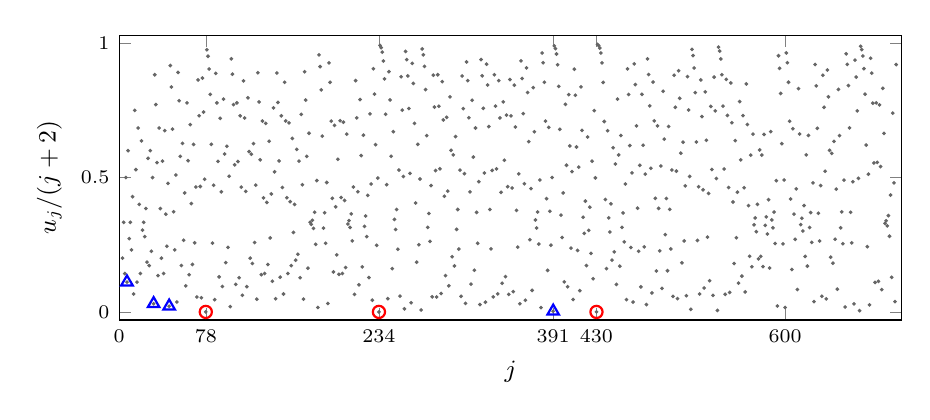
\begin{tikzpicture}
\begin{axis}[width=0.95\textwidth,height=5.2cm,xmin=0,xmax=705,ymin=-0.03,ymax=1.03,
  xlabel={$j$},ylabel={$u_j/(j+2)$},tick label style={font=\scriptsize},label style={font=\small},
  xtick={0,78,234,391,430,600},ytick={0,0.5,1}]
\addplot[only marks,mark=*,mark size=0.45pt,black!60] coordinates {(3,0.2000) (4,0.3333) (5,0.1429) (6,0.5000) (7,0.1111) (8,0.6000) (9,0.2727) (10,0.3333) (11,0.2308) (12,0.4286) (13,0.0667) (14,0.7500) (15,0.5294) (16,0.1111) (17,0.6842) (18,0.4000) (19,0.1429) (20,0.6364) (21,0.3043) (22,0.3333) (23,0.2800) (24,0.3846) (25,0.1852) (26,0.5714) (27,0.1724) (28,0.6000) (29,0.2258) (30,0.5000) (31,0.0303) (32,0.8824) (33,0.7714) (34,0.5556) (35,0.1351) (36,0.6842) (37,0.3846) (38,0.2000) (39,0.5610) (40,0.1429) (41,0.6744) (42,0.3636) (43,0.2444) (44,0.4783) (45,0.0213) (46,0.9167) (47,0.8367) (48,0.6800) (49,0.3725) (50,0.2308) (51,0.5094) (52,0.0370) (53,0.8909) (54,0.7857) (55,0.5789) (56,0.1724) (57,0.6271) (58,0.2667) (59,0.4426) (60,0.0968) (61,0.7778) (62,0.5625) (63,0.1385) (64,0.6970) (65,0.4030) (66,0.1765) (67,0.6232) (68,0.2571) (69,0.4648) (70,0.0556) (71,0.8630) (72,0.7297) (73,0.4667) (74,0.0526) (75,0.8701) (76,0.7436) (77,0.4937) (78,0.0000) (79,0.9753) (80,0.9512) (81,0.9036) (82,0.8095) (83,0.6235) (84,0.2558) (85,0.4713) (86,0.0455) (87,0.8876) (88,0.7778) (89,0.5604) (90,0.1304) (91,0.7204) (92,0.4468) (93,0.0947) (94,0.7917) (95,0.5876) (96,0.1837) (97,0.6162) (98,0.2400) (99,0.5050) (100,0.0196) (101,0.9417) (102,0.8846) (103,0.7714) (104,0.5472) (105,0.1028) (106,0.7778) (107,0.5596) (108,0.1273) (109,0.7297) (110,0.4643) (111,0.0619) (112,0.8596) (113,0.7217) (114,0.4483) (115,0.0940) (116,0.7966) (117,0.5966) (118,0.2000) (119,0.5868) (120,0.1803) (121,0.6260) (122,0.2581) (123,0.4720) (124,0.0476) (125,0.8898) (126,0.7812) (127,0.5659) (128,0.1385) (129,0.7099) (130,0.4242) (131,0.1429) (132,0.7015) (133,0.4074) (134,0.1765) (135,0.6350) (136,0.2754) (137,0.4388) (138,0.1143) (139,0.7589) (140,0.5211) (141,0.0490) (142,0.8889) (143,0.7793) (144,0.5616) (145,0.1293) (146,0.7297) (147,0.4631) (148,0.0667) (149,0.8543) (150,0.7105) (151,0.4248) (152,0.1429) (153,0.7032) (154,0.4103) (155,0.1720) (156,0.6456) (157,0.2956) (158,0.4000) (159,0.1925) (160,0.6049) (161,0.2147) (162,0.5610) (163,0.1273) (164,0.7349) (165,0.4731) (166,0.0476) (167,0.8935) (168,0.7882) (169,0.5789) (170,0.1628) (171,0.6647) (172,0.3333) (173,0.3257) (174,0.3409) (175,0.3107) (176,0.3708) (177,0.2514) (178,0.4889) (179,0.0166) (180,0.9560) (181,0.9126) (182,0.8261) (183,0.6541) (184,0.3118) (185,0.3690) (186,0.2553) (187,0.4815) (188,0.0316) (189,0.9267) (190,0.8542) (191,0.7098) (192,0.4227) (193,0.1487) (194,0.6939) (195,0.3909) (196,0.2121) (197,0.5678) (198,0.1400) (199,0.7114) (200,0.4257) (201,0.1429) (202,0.7059) (203,0.4146) (204,0.1650) (205,0.6618) (206,0.3269) (207,0.3397) (208,0.3143) (209,0.3649) (210,0.2642) (211,0.4648) (212,0.0654) (213,0.8605) (214,0.7222) (215,0.4470) (216,0.1009) (217,0.7900) (218,0.5818) (219,0.1674) (220,0.6577) (221,0.3184) (222,0.3571) (223,0.2800) (224,0.4336) (225,0.1278) (226,0.7368) (227,0.4760) (228,0.0435) (229,0.9048) (230,0.8103) (231,0.6223) (232,0.2479) (233,0.4979) (234,0.0000) (235,0.9916) (236,0.9832) (237,0.9665) (238,0.9333) (239,0.8672) (240,0.7355) (241,0.4733) (242,0.0492) (243,0.8939) (244,0.7886) (245,0.5789) (246,0.1613) (247,0.6707) (248,0.3440) (249,0.3068) (250,0.3810) (251,0.2332) (252,0.5276) (253,0.0588) (254,0.8750) (255,0.7510) (256,0.5039) (257,0.0116) (258,0.9692) (259,0.9387) (260,0.8779) (261,0.7567) (262,0.5152) (263,0.0340) (264,0.9248) (265,0.8502) (266,0.7015) (267,0.4052) (268,0.1852) (269,0.6236) (270,0.2500) (271,0.4945) (272,0.0073) (273,0.9782) (274,0.9565) (275,0.9134) (276,0.8273) (277,0.6559) (278,0.3143) (279,0.3665) (280,0.2624) (281,0.4700) (282,0.0563) (283,0.8807) (284,0.7622) (285,0.5261) (286,0.0556) (287,0.8824) (288,0.7655) (289,0.5326) (290,0.0685) (291,0.8567) (292,0.7143) (293,0.4305) (294,0.1351) (295,0.7239) (296,0.4497) (297,0.0970) (298,0.8000) (299,0.6013) (300,0.2053) (301,0.5842) (302,0.1711) (303,0.6525) (304,0.3072) (305,0.3811) (306,0.2338) (307,0.5275) (308,0.0581) (309,0.8778) (310,0.7564) (311,0.5144) (312,0.0318) (313,0.9302) (314,0.8608) (315,0.7224) (316,0.4465) (317,0.1034) (318,0.7875) (319,0.5763) (320,0.1553) (321,0.6842) (322,0.3704) (323,0.2554) (324,0.4847) (325,0.0275) (326,0.9390) (327,0.8784) (328,0.7576) (329,0.5166) (330,0.0361) (331,0.9219) (332,0.8443) (333,0.6896) (334,0.3810) (335,0.2344) (336,0.5266) (337,0.0560) (338,0.8824) (339,0.7654) (340,0.5322) (341,0.0671) (342,0.8605) (343,0.7217) (344,0.4451) (345,0.1066) (346,0.7816) (347,0.5645) (348,0.1314) (349,0.7322) (350,0.4659) (351,0.0652) (352,0.8644) (353,0.7296) (354,0.4607) (355,0.0756) (356,0.8436) (357,0.6880) (358,0.3778) (359,0.2410) (360,0.5138) (361,0.0303) (362,0.9341) (363,0.8685) (364,0.7377) (365,0.4768) (366,0.0435) (367,0.9079) (368,0.8162) (369,0.6334) (370,0.2688) (371,0.4584) (372,0.0802) (373,0.8347) (374,0.6702) (375,0.3422) (376,0.3122) (377,0.3720) (378,0.2526) (379,0.4908) (380,0.0157) (381,0.9634) (382,0.9271) (383,0.8545) (384,0.7098) (385,0.4212) (386,0.1546) (387,0.6864) (388,0.3744) (389,0.2481) (390,0.5000) (391,0.0025) (392,0.9898) (393,0.9797) (394,0.9596) (395,0.9194) (396,0.8392) (397,0.6792) (398,0.3600) (399,0.2768) (400,0.4428) (401,0.1117) (402,0.7723) (403,0.5457) (404,0.0936) (405,0.8084) (406,0.6176) (407,0.2372) (408,0.5220) (409,0.0462) (410,0.9029) (411,0.8063) (412,0.6135) (413,0.2289) (414,0.5385) (415,0.0791) (416,0.8373) (417,0.6754) (418,0.3524) (419,0.2922) (420,0.4123) (421,0.1726) (422,0.6509) (423,0.3035) (424,0.3897) (425,0.2178) (426,0.5607) (427,0.1235) (428,0.7488) (429,0.4988) (430,0.0000) (431,0.9954) (432,0.9908) (433,0.9816) (434,0.9633) (435,0.9268) (436,0.8539) (437,0.7084) (438,0.4182) (439,0.1610) (440,0.6742) (441,0.3499) (442,0.2973) (443,0.4022) (444,0.1928) (445,0.6107) (446,0.2232) (447,0.5501) (448,0.1022) (449,0.7916) (450,0.5841) (451,0.1700) (452,0.6564) (453,0.3143) (454,0.3684) (455,0.2604) (456,0.4760) (457,0.0458) (458,0.9043) (459,0.8091) (460,0.6190) (461,0.2397) (462,0.5172) (463,0.0366) (464,0.9227) (465,0.8458) (466,0.6923) (467,0.3859) (468,0.2255) (469,0.5456) (470,0.0932) (471,0.8097) (472,0.6203) (473,0.2421) (474,0.5126) (475,0.0273) (476,0.9414) (477,0.8831) (478,0.7667) (479,0.5343) (480,0.0705) (481,0.8551) (482,0.7107) (483,0.4227) (484,0.1523) (485,0.6920) (486,0.3852) (487,0.2270) (488,0.5429) (489,0.0876) (490,0.8211) (491,0.6430) (492,0.2874) (493,0.4222) (494,0.1532) (495,0.6901) (496,0.3815) (497,0.2345) (498,0.5280) (499,0.0579) (500,0.8805) (501,0.7614) (502,0.5238) (503,0.0495) (504,0.8972) (505,0.7949) (506,0.5906) (507,0.1827) (508,0.6314) (509,0.2642) (510,0.4688) (511,0.0604) (512,0.8755) (513,0.7515) (514,0.5039) (515,0.0097) (516,0.9768) (517,0.9538) (518,0.9077) (519,0.8157) (520,0.6322) (521,0.2658) (522,0.4656) (523,0.0667) (524,0.8631) (525,0.7268) (526,0.4545) (527,0.0888) (528,0.8189) (529,0.6384) (530,0.2782) (531,0.4409) (532,0.1161) (533,0.7645) (534,0.5299) (535,0.0615) (536,0.8736) (537,0.7477) (538,0.4963) (539,0.0055) (540,0.9852) (541,0.9705) (542,0.9412) (543,0.8826) (544,0.7656) (545,0.5320) (546,0.0657) (547,0.8652) (548,0.7309) (549,0.4628) (550,0.0725) (551,0.8517) (552,0.7040) (553,0.4090) (554,0.1799) (555,0.6373) (556,0.2760) (557,0.4454) (558,0.1071) (559,0.7825) (560,0.5658) (561,0.1332) (562,0.7305) (563,0.4619) (564,0.0742) (565,0.8483) (566,0.6972) (567,0.3954) (568,0.2070) (569,0.5832) (570,0.1678) (571,0.6614) (572,0.3240) (573,0.3496) (574,0.2986) (575,0.4003) (576,0.1972) (577,0.6028) (578,0.2069) (579,0.5835) (580,0.1684) (581,0.6604) (582,0.3219) (583,0.3538) (584,0.2901) (585,0.4174) (586,0.1633) (587,0.6706) (588,0.3424) (589,0.3130) (590,0.3716) (591,0.2546) (592,0.4882) (593,0.0218) (594,0.9530) (595,0.9062) (596,0.8127) (597,0.6260) (598,0.2533) (599,0.4908) (600,0.0166) (601,0.9635) (602,0.9272) (603,0.8545) (604,0.7096) (605,0.4201) (606,0.1579) (607,0.6814) (608,0.3639) (609,0.2700) (610,0.4575) (611,0.0832) (612,0.8306) (613,0.6618) (614,0.3247) (615,0.3485) (616,0.3010) (617,0.3958) (618,0.2065) (619,0.5845) (620,0.1704) (621,0.6565) (622,0.3141) (623,0.3696) (624,0.2588) (625,0.4801) (626,0.0382) (627,0.9205) (628,0.8413) (629,0.6830) (630,0.3671) (631,0.2638) (632,0.4700) (633,0.0583) (634,0.8805) (635,0.7614) (636,0.5235) (637,0.0485) (638,0.9000) (639,0.8003) (640,0.6012) (641,0.2037) (642,0.5901) (643,0.1814) (644,0.6347) (645,0.2705) (646,0.4568) (647,0.0847) (648,0.8277) (649,0.6559) (650,0.3129) (651,0.3721) (652,0.2538) (653,0.4901) (654,0.0183) (655,0.9604) (656,0.9210) (657,0.8422) (658,0.6848) (659,0.3707) (660,0.2568) (661,0.4842) (662,0.0301) (663,0.9368) (664,0.8739) (665,0.7481) (666,0.4970) (667,0.0045) (668,0.9881) (669,0.9762) (670,0.9524) (671,0.9049) (672,0.8101) (673,0.6207) (674,0.2426) (675,0.5126) (676,0.0265) (677,0.9440) (678,0.8882) (679,0.7768) (680,0.5543) (681,0.1098) (682,0.7778) (683,0.5562) (684,0.1137) (685,0.7700) (686,0.5407) (687,0.0827) (688,0.8319) (689,0.6643) (690,0.3295) (691,0.3391) (692,0.3199) (693,0.3583) (694,0.2816) (695,0.4347) (696,0.1289) (697,0.7396) (698,0.4800) (699,0.0385) (700,0.9202)};
\addplot[only marks,mark=o,mark size=2.2pt,red,thick] coordinates {(78,0) (234,0) (430,0)};
\addplot[only marks,mark=triangle,mark size=2.4pt,blue,thick] coordinates {(391,0.0025) (7,0.111) (31,0.0303) (45,0.0213)};
\end{axis}
\end{tikzpicture}
\caption{The tent sequence of $n=3$, normalised as $u_j/(j+2)\in[0,1]$, for $3\le j\le700$. Circles: centres ($u_j=0$) at $78,234,430$; triangles: odd windows at which solutions end ($j=7,31,45$ on the lower side before the first centre, and $j=391$, giving $a_k=392$). The normalised sequence follows the tent map $t\mapsto|2t-1|$ up to $O(1/j)$; branching and termination happen only in the windows $u_j\le1$.}\label{fig:tent}
\end{figure}

\begin{example}\label{ex:n3}
For $n=3$ the tent sequence has odd windows at $3,5,7,13,31,45$ before its first centre $78$; the unique path has offset $-1$ at $7,31,45$, giving the solutions with $a_k=8,32,46$ (with $3,15,23$ terms). The next centres are $234,430,1502,2942,6058,6618,18910,54222$ and the next odd windows $391,12229,55327,155941$. At $K-1=391$ we have $h=2$: $A_0=37$ inclusions on $[3,78)$, the block $[78,234)$ has $L_1=156$ and $x_1\in\{75,81\}$, and the final segment contributes $y=72$. So the two solutions with $a_k=392$ have $1+37+72+\{75,81\}=\{185,191\}$ terms. Figure~\ref{fig:tent} shows the beginning of this tent sequence.
\end{example}

\section{The upper inequality of Conjecture 3.7 is false}\label{sec:counter}

\noindent\begin{minipage}{\textwidth}
Let $A^*$ be the set consisting of the following $185$ integers:
\begin{center}\begin{minipage}{0.94\textwidth}\small\raggedright
4, 6, 9, 10, 12, 14, 18, 19, 21, 22, 24, 26, 29, 30, 33, 34, 35, 36, 39, 42, 43, 45, 47, 48, 49, 50, 52, 53, 58, 59, 61, 65, 66, 68, 69, 71, 75, 80, 81, 82, 83, 84, 85, 87, 92, 93, 95, 96, 97, 100, 101, 107, 108, 109, 112, 116, 120, 121, 124, 126, 127, 128, 129, 132, 135, 138, 140, 141, 142, 147, 148, 150, 151, 152, 154, 155, 157, 158, 160, 163, 164, 167, 172, 173, 175, 177, 179, 181, 182, 183, 184, 185, 187, 189, 194, 197, 200, 201, 203, 204, 206, 207, 209, 211, 213, 217, 221, 222, 224, 226, 229, 234, 235, 243, 248, 249, 251, 253, 254, 259, 260, 261, 262, 263, 264, 269, 272, 274, 275, 276, 277, 278, 279, 281, 283, 288, 289, 290, 291, 295, 298, 302, 303, 306, 308, 309, 314, 315, 316, 317, 319, 320, 321, 324, 326, 332, 333, 334, 335, 337, 338, 343, 344, 345, 347, 348, 349, 352, 356, 360, 363, 364, 365, 366, 368, 369, 370, 371, 373, 377, 379, 381, 387, 390, 392.
\end{minipage}\end{center}
\end{minipage}

In run notation, $A^*$ consists of the $101$ maximal runs
$4$, $6$, $9$--$10$, $12$, $14$, $18$--$19$, $21$--$22$, $24$, $26$, $29$--$30$, $33$--$36$, $39$, $42$--$43$, $45$, $47$--$50$, $52$--$53$, $58$--$59$, $61$, $65$--$66$, $68$--$69$, $71$, $75$, $80$--$85$, $87$, $92$--$93$, $95$--$97$, $100$--$101$, $107$--$109$, $112$, $116$, $120$--$121$, $124$, $126$--$129$, $132$, $135$, $138$, $140$--$142$, $147$--$148$, $150$--$152$, $154$--$155$, $157$--$158$, $160$, $163$--$164$, $167$, $172$--$173$, $175$, $177$, $179$, $181$--$185$, $187$, $189$, $194$, $197$, $200$--$201$, $203$--$204$, $206$--$207$, $209$, $211$, $213$, $217$, $221$--$222$, $224$, $226$, $229$, $234$--$235$, $243$, $248$--$249$, $251$, $253$--$254$, $259$--$264$, $269$, $272$, $274$--$279$, $281$, $283$, $288$--$291$, $295$, $298$, $302$--$303$, $306$, $308$--$309$, $314$--$317$, $319$--$321$, $324$, $326$, $332$--$335$, $337$--$338$, $343$--$345$, $347$--$349$, $352$, $356$, $360$, $363$--$366$, $368$--$371$, $373$, $377$, $379$, $381$, $387$, $390$, $392$.

\begin{theorem}\label{thm:counter}
\begin{enumerate}[label=\textup{(\alph*)}]
\item $\sum_{a\in A^*}a\,2^{-a}=3/8$, $|A^*|=185$, $\min A^*=4$ and $\max A^*=392$. Hence $(n,k,a_k)=(3,185,392)$ solves \eqref{eq:EG} and $a_k=392>376=2(k+n)$.
\item Equation \eqref{eq:EG} has exactly $403$ solutions with $a_k\le392$. Exactly $37$ of them violate $a_k\le2(k+n)$; all of these have $a_k=392$, and they are listed in Table~\ref{tab:392}. In particular $392$ is the least largest term of a counterexample.
\item Every solution with $k\le176$ satisfies $a_k\le2(k+n)$. The only counterexample with $k=177$ is $n=18$, $a_k=392$. There is no counterexample with $392<a_k<12230$, and there are counterexamples with $a_k=12230$ for $61$ values of $n$.
\item For $n=3$, the values of $a_k\le 2\cdot10^9$ for which solutions exist, their numbers, and the least and largest $k$ are given in Table~\ref{tab:n3}. In particular the excess $a_k-2(n+k)$ of the solution with fewest terms is positive for $a_k=392$, $12230$, $55328$, $155942$, $460536$, $3254286$, $7466440$, $7729366$, $10096672$, $11898120$ and $753950542$, and equals $21300$ for $a_k=753950542$.
\item For every $n\le 16513$ there is a counterexample with this $n$ and $a_k\le 753950542$; for $n\le3000$ one with $a_k\le7729366$.
\end{enumerate}
\end{theorem}

\begin{proof}
(a) Multiplying by $2^{392}$, the claim is the integer identity $3\cdot2^{389}=\sum_{a\in A^*}a\,2^{392-a}$, which we checked exactly with three independent systems (Section~\ref{sec:cert}). It can also be checked by hand through Lemma~\ref{lem:states}: starting from $\rho_3=3$ and applying $\rho_{j+1}=2\rho_j-(j+1)[\,j+1\in A^*]$ for $j=3,\dots,391$, all states stay in $[1,j+1]$ and $\rho_{392}=0$.

(b) If $a_k\le392$ then $n<392$ by Lemma~\ref{lem:a1}. For each $n\le391$, by Lemma~\ref{lem:states} the solutions with $a_k\le392$ are exactly the $0/1$-sequences whose states stay live until they reach $0$ at some time $K\le392$. We enumerated them by dynamic programming over the pairs (state, number of inclusions), without using Section~\ref{sec:tent}; at every time at most two states occurred, as Theorem~\ref{thm:rigid} predicts.

(c) Let $(n;A)$ be a counterexample, $K=a_k$, $E=K-n-k$. Then $K>2(n+k)$ means $E>n+k$, so $K=n+k+E<2E\le 2k\lfloor\log_2K\rfloor$ and $n<E-k\le k(\lfloor\log_2K\rfloor-1)$ by Lemma~\ref{lem:gap}. If $k\le177$, then $K<354\lfloor\log_2K\rfloor$; this is impossible for $K\ge8192$, and for $K<8192$ it gives $K<354\cdot12=4248$. Hence $\lfloor\log_2 K\rfloor\le12$ and $n<177\cdot11=1947$. Also, every counterexample with $K\le5000$ has $n+k<K/2\le2500$. An exhaustive search as in (b) over all $n\le2500$ and $K\le5000$, keeping all cardinalities below $2600$, finds no counterexample other than the $37$ of Table~\ref{tab:392}; their least $k$ is $177$, attained only for $n=18$. For $5000<K<12230$ and $K=12230$ we used Theorem~\ref{thm:blocks}: a counterexample with largest term $K$ has $n<K/2$, and for each such $n$ Corollary~\ref{cor:alg} gives the least cardinality at every odd window up to $12229$.

(d) Corollary~\ref{cor:alg} with $n=3$, $J=2\cdot10^9$; the values for $K\le155942$ were also confirmed by the dynamic programming of (b).

(e) For $n\le3000$: Corollary~\ref{cor:alg}, run for each $n$ until the least cardinality at some odd window violates the inequality. For all $n\le16513$: the tent sequence of $n$ coincides with that of $3$ from some time $t_n\le n+52301$ on; up to $t_n$ we compute, for each of the at most two live states of Theorem~\ref{thm:rigid}, the least number of inclusions of a path of $n$ reaching it, and after $t_n$ we combine it with the block data of $n=3$ (Theorem~\ref{thm:blocks}) at every odd window of $n=3$ up to $753950541$. Here the two live states at time $t_n$ have opposite offsets, so up to the next centre they follow the reference path of $n=3$ and its mirror image, whose inclusion counts are $P$ and $L-P$ ($P$ the count of the reference path, $L$ the length); from that centre on, the block minima of $n=3$ apply. Both procedures give the same least counterexample for every $n\le3000$. An independent implementation that does not use Section~\ref{sec:tent} (a least-count dynamic programming for each $n$ up to a common time $T$, followed by one dynamic programming started from the union of the states reached at time $T$) confirmed (e) and showed that $n=16514$ has no counterexample with $a_k\le2\cdot10^9$.
\end{proof}

\begin{table}[ht]
\centering\small
\begin{tabular}{r r r r @{\qquad} r r r r}
\toprule
$n$ & $k$ & $\#$ & $a_k-2(n+k)$ & $n$ & $k$ & $\#$ & $a_k-2(n+k)$\\
\midrule
1 & 185 & 1 & 20 & 6 & 185 & 1 & 10\\
1 & 187 & 1 & 16 & 7 & 183 & 4 & 12\\
1 & 191 & 1 & 8 & 7 & 185 & 4 & 8\\
1 & 193 & 1 & 4 & 8 & 183 & 1 & 10\\
2 & 185 & 1 & 18 & 9 & 184 & 1 & 6\\
2 & 187 & 1 & 14 & 10 & 183 & 1 & 6\\
2 & 191 & 1 & 6 & 11 & 183 & 1 & 4\\
2 & 193 & 1 & 2 & 12 & 182 & 4 & 4\\
3 & 185 & 1 & 16 & 13 & 182 & 2 & 2\\
3 & 191 & 1 & 4 & 14 & 181 & 1 & 2\\
4 & 186 & 1 & 12 & 16 & 179 & 2 & 2\\
5 & 185 & 2 & 12 & 17 & 178 & 1 & 2\\
  &     &   &    & 18 & 177 & 1 & 2\\
\bottomrule
\end{tabular}
\caption{All solutions of \eqref{eq:EG} with $a_k\le 392$ that violate $a_k\le 2(k+n)$. All have $a_k=392$; $\#$ is the number of solutions with the given $(n,k)$; in total $37$ solutions.}\label{tab:392}
\end{table}

\begin{table}[ht]
\centering\small
\begin{tabular}{r r r r r r}
\toprule
$K=a_k$ & $h$ & $\#$sol. & $k_{\min}$ & $k_{\max}$ & $K-2(3+k_{\min})$\\
\midrule
8 & 0 & 1 & 3 & 3 & $-4$\\
32 & 0 & 1 & 15 & 15 & $-4$\\
46 & 0 & 1 & 23 & 23 & $-6$\\
392 & 2 & $2^{1}$ & 185 & 191 & 16\\
12230 & 7 & $2^{6}$ & 6079 & 6163 & 66\\
55328 & 9 & $2^{8}$ & 27570 & 27760 & 182\\
155942 & 9 & $2^{8}$ & 77814 & 78004 & 308\\
460536 & 9 & $2^{8}$ & 229624 & 229814 & 1282\\
659488 & 9 & $2^{8}$ & 330013 & 330203 & $-544$\\
1025582 & 9 & $2^{8}$ & 512985 & 513175 & $-394$\\
1047128 & 9 & $2^{8}$ & 523845 & 524035 & $-568$\\
3254286 & 9 & $2^{8}$ & 1626358 & 1626548 & 1564\\
3437088 & 9 & $2^{8}$ & 1718933 & 1719123 & $-784$\\
7466440 & 9 & $2^{8}$ & 3731892 & 3732082 & 2650\\
7729366 & 9 & $2^{8}$ & 3863049 & 3863239 & 3262\\
10096672 & 9 & $2^{8}$ & 5047226 & 5047416 & 2214\\
11898120 & 9 & $2^{8}$ & 5948065 & 5948255 & 1984\\
753950542 & 10 & $2^{9}$ & 376964618 & 376967062 & 21300\\
1449322158 & 10 & $2^{9}$ & 724681507 & 724683951 & $-40862$\\
1452777560 & 10 & $2^{9}$ & 726410287 & 726412731 & $-43020$\\
1691887144 & 10 & $2^{9}$ & 845953762 & 845956206 & $-20386$\\
\bottomrule
\end{tabular}
\caption{All representations $3/8=\sum_{a\in A}a2^{-a}$ with $A\subseteq\Z_{>3}$ $($i.e.\ all solutions of \eqref{eq:EG} for $n=3)$ and $\max A=K\le 2\cdot 10^9$: $h$ is the number of centres before $K-1$, $k_{\min},k_{\max}$ the least and largest $|A|$.}\label{tab:n3}
\end{table}

\begin{remark}[why greedy data supported the conjecture]
By Theorem~\ref{thm:blocks}, the cardinalities of the representations with a given largest term $K$ spread around $K/2$, and the spread grows with the number of centres. A conjecture of the form $a_k\le2(k+n)$, i.e.\ $k\ge K/2-n$, is therefore about the \emph{least} cardinality, while one greedy representation per $n$ samples a single choice at every centre. For $n=14$ the greedy representation has $187$ terms, the least one $181$.
\end{remark}

\section{The bound in terms of \texorpdfstring{$k$}{k}: the true half of Conjecture 3.7}\label{sec:sharp}

\begin{theorem}\label{thm:sharp}
Every solution of \eqref{eq:EG} satisfies $a_k\le2^{k+1}-2$, with equality if and only if $n=2^{k+1}-k-2$ and $a_i=n+i$ $(1\le i\le k)$.
\end{theorem}

\begin{proof}
Let $K=a_k$ and $E=K-n-k\ge0$ (Lemma~\ref{lem:a1}); $E$ is the number of integers in $(n,K]$ missing from $A$.

\emph{Case $E=0$.} Then $A=\{n+1,\dots,n+k\}$ and $n=\sum_{i=1}^k(n+i)2^{-i}=n+2-(n+k+2)2^{-k}$, so $n=2^{k+1}-k-2$ and $K=2^{k+1}-2$.

\emph{Case $1\le E\le 2^{k-1}-1$.} Since $1-2^{-E-1}\ge\frac34$, Lemma~\ref{lem:extremal} gives
$K\le\frac43(2^k+E-1)\le\frac43(3\cdot2^{k-1}-2)=2^{k+1}-\frac83<2^{k+1}-2$.

\emph{Case $E\ge2^{k-1}$.} Then $E\ge k$, hence $2^{E+1}\ge 2^k+2^E>2^k+E$, and Lemma~\ref{lem:extremal} gives
\[
K\le\frac{2^k+E-1}{1-2^{-E-1}}=(2^k+E-1)\Bigl(1+\frac{1}{2^{E+1}-1}\Bigr)<2^k+E,
\]
so $K\le2^k+E-1$. Suppose $K\ge2^{k+1}-2$. Then $E\ge2^k-1$, so $2^k+E\le 2E+1$, and Lemma~\ref{lem:gap} gives $E\le k\log_2K<k\log_2(2E+1)$. The function $\varphi(t)=t/\log_2(2t+1)$ is increasing for $t\ge1$, since $\ln(2t+1)>\frac{2t}{2t+1}$. Hence $k>\varphi(E)\ge\varphi(2^k-1)$, i.e.\ $2^k-1<k\log_2(2^{k+1}-1)<k(k+1)$. This is false for $k\ge5$. So for $k\ge5$ this case gives $K\le2^{k+1}-3$.

\emph{Small $k$.} For $k\le4$, Lemma~\ref{lem:extremal} gives $n\le26$ and Lemma~\ref{lem:gap} gives $K\le 30+4\lfloor\log_2K\rfloor$, hence $K\le50$. An exhaustive search over $n\le26$, $K\le50$ (Section~\ref{sec:Nk}) shows that the solutions with $k\le4$ are $(4;5,6)$; $(1;3,6,8)$, $(2;3,6,8)$, $(1;4,5,6)$, $(2;4,5,6)$, $(3;4,6,8)$, $(11;12,13,14)$; $(9;10,11,13,14)$, $(26;27,28,29,30)$, in agreement with \cite[Thm.~2.5]{TUZ}. Their largest terms obey the theorem.
\end{proof}

\begin{corollary}\label{cor:half}
Every solution satisfies $a_k\le 2(2^k-1)=\frac12\cdot 4(2^k-1)$. Thus the ``in particular'' clause of Conjecture~3.7 holds, although the inequality $a_k\le 2(k+n)$ from which it was derived fails. The bound $2^{k+1}-2$ is attained for every $k$ and improves \eqref{eq:TUZbound} by a factor tending to $2$.
\end{corollary}

The upper inequality of Conjecture~3.7 does hold outside a thin range. \cite[Rem.~3.8]{TUZ} proves it for $n\ge2^k-k$; the gap lemma gives a much larger region.

\begin{proposition}\label{prop:region}
Every solution of \eqref{eq:EG} with $a_k>2(k+n)$ satisfies
\[
a_k<2k\lfloor\log_2a_k\rfloor,\qquad a_k<4k\log_2(4k),\qquad n<k\bigl(\lfloor\log_2a_k\rfloor-1\bigr)<k\bigl(1+\log_2k+\log_2\log_2(4k)\bigr).
\]
Consequently $a_k\le2(k+n)$ holds whenever $k\le176$ or $n\ge k\bigl(1+\log_2k+\log_2\log_2(4k)\bigr)$; in particular whenever $n\ge 2k\log_2(4k)$.
\end{proposition}

\begin{proof}
Let $K=a_k$ and $E=K-n-k$. The assumption $K>2(n+k)$ means $E>n+k$, i.e.\ $n+k<K/2<E$. By Lemma~\ref{lem:gap}, $K<2E\le2k\lfloor\log_2K\rfloor$ and $n<E-k\le k(\lfloor\log_2K\rfloor-1)$. If $K\ge K_0:=4k\log_2(4k)$, then, since $t/\log_2t$ is increasing for $t\ge e$,
$K/\log_2K\ge K_0/\log_2K_0=4k\log_2(4k)/\bigl(\log_2(4k)+\log_2\log_2(4k)\bigr)\ge2k$, contradicting $K<2k\log_2K$. Hence $K<K_0$ and $\lfloor\log_2K\rfloor-1<\log_2K_0-1=1+\log_2k+\log_2\log_2(4k)$. The case $k\le176$ is Theorem~\ref{thm:counter}(c), and $1+\log_2k+\log_2\log_2(4k)\le2\log_2(4k)$ because $\log_2\log_2(4k)\le 3+\log_2 k$.
\end{proof}

\begin{remark}
Thus the counterexamples live in the range $n<k(1+\log_2k+\log_2\log_2(4k))$, $a_k<4k\log_2(4k)$, as opposed to the exponential range $n<2^k-k$ left open in \cite{TUZ}. All counterexamples we found have $n$ much smaller than $k$; for instance $n=16513$, $k=376956377$, $a_k=753950542$.
\end{remark}

\section{All solutions with at most 28 terms}\label{sec:Nk}

Let $N(k)$ be the number of solutions of \eqref{eq:EG} with exactly $k$ terms (all $n\ge1$). By Lemma~\ref{lem:extremal}, $n\le2^{k+1}-k-2$, and by Lemma~\ref{lem:gap}, $a_k\le n+k(1+\log_2a_k)$. For each $n$ in this range we ran the dynamic programming of Theorem~\ref{thm:counter}(b), keeping for each state the vector of the numbers of paths with $0,1,\dots,k_{\max}-1$ inclusions, until the gap bound excludes further solutions. A second program first tests, using Theorem~\ref{thm:count}(iii), whether the tent sequence has an odd window in the relevant range, and runs the same dynamic programming only for such $n$; the two programs produced identical lists of solutions for $k\le 22$. The complete list of the $252$ solutions with $k\le28$ is in the supplementary archive (file \texttt{solutions\_k\_le\_28.txt}); it was also reproduced by an independent program.

\begin{theorem}\label{thm:Nk}
For $2\le k\le28$, the values of $N(k)$ and the least largest term $\min a_k$ are as in Table~\ref{tab:Nk}. For each $k$ the largest $a_k$ is $2^{k+1}-2$, attained only by the consecutive solution.
\end{theorem}

\begin{table}[ht]
\centering\small
\begin{tabular}{r r r @{\qquad} r r r}
\toprule
$k$ & $N(k)$ & $\min a_k$ & $k$ & $N(k)$ & $\min a_k$\\
\midrule
2 & 1 & 6 & 16 & 12 & 46\\
3 & 6 & 6 & 17 & 12 & 46\\
4 & 2 & 14 & 18 & 10 & 88\\
5 & 4 & 14 & 19 & 6 & 70\\
6 & 5 & 14 & 20 & 13 & 46\\
7 & 5 & 14 & 21 & 11 & 46\\
8 & 5 & 32 & 22 & 11 & 70\\
9 & 5 & 24 & 23 & 20 & 46\\
10 & 7 & 128 & 24 & 16 & 406\\
11 & 3 & 184 & 25 & 14 & 1536\\
12 & 5 & 104 & 26 & 12 & 406\\
13 & 14 & 32 & 27 & 19 & 544\\
14 & 7 & 46 & 28 & 16 & 320\\
15 & 11 & 32 & & & \\
\bottomrule
\end{tabular}
\caption{Number $N(k)$ of solutions of \eqref{eq:EG} with exactly $k$ terms, and the least value of $a_k$ among them.}\label{tab:Nk}
\end{table}

\begin{remark}[corrections to \cite{TUZ}]
For $k=8$ the list in \cite[Thm.~2.5]{TUZ} contains $n=17,19,197,502$ but not
\[
\frac{35}{2^{35}}=\frac{36}{2^{36}}+\frac{37}{2^{37}}+\frac{38}{2^{38}}+\frac{39}{2^{39}}+\frac{42}{2^{42}}+\frac{43}{2^{43}}+\frac{45}{2^{45}}+\frac{46}{2^{46}},
\]
which one checks by hand: $35\cdot2^{11}=71680=36\cdot2^{10}+37\cdot2^9+38\cdot2^8+39\cdot2^7+42\cdot2^4+43\cdot2^3+45\cdot2+46$. Hence $N(8)=5$. For $k=7$ the list in \cite[Thm.~2.5]{TUZ} has five solutions, in agreement with Table~\ref{tab:Nk}, while the text of \cite[\S3]{TUZ} states $N(7)=3$.
\end{remark}

\begin{remark}[large values of $N(k)$]
\cite[Conj.~3.3]{TUZ} asserts $\limsup N(k)=\infty$; \cite[Prop.~3.1]{TUZ} gives $N(k)\ge5$ for $k$ in an explicit residue class. Theorem~\ref{thm:blocks} produces many solutions with the same $k$ and the same $a_k$ for different $n$: counting all solutions with $a_k=392$, $12230$, $55328$ and $155942$ (for all $n<a_k$) gives
\[
N(185)\ge14,\qquad N(6109)\ge122,\qquad N(27612)\ge274,\qquad N(77856)\ge274 .
\]
The first bound was also obtained by the dynamic programming of Theorem~\ref{thm:counter}(b). For $k=185$ and $k=6109$ we also constructed the $14$, respectively $122$, solutions explicitly and verified each identity by exact integer arithmetic.
\end{remark}

\section{Consequences for Erd\H{o}s Problem \texorpdfstring{\#261}{261}}\label{sec:261}

\begin{corollary}\label{cor:ii}
Let $n\ge1$ and let $(u_j)_{j\ge n}$ be the tent sequence with $u_n=|n-2|$. Then \eqref{eq:EG} is solvable for this $n$ if and only if there is an odd window $j\ge n$, $(n,j)\ne(1,1)$, such that either $c(j)\ge1$, or $c(j)=0$ and the unique live path has offset $-1$ at time $j$.
\end{corollary}

\begin{proof}
Theorem~\ref{thm:count}(iii) with $N=n$; the excluded case is the one-term representation $\frac12=\frac{2}{2^2}$. For $n\ge2$ every representation of $n/2^n$ by integers $>n$ has at least two terms, since $f(K)=f(n)$ with $K>n$ is impossible.
\end{proof}

Thus the second question of Problem \#261 asks whether every tent sequence started at $u_n=|n-2|$ reaches such a configuration, and the termination conjecture of Borwein and Loring asks the same for the greedy path. Using Corollary~\ref{cor:ii} we checked:

\begin{proposition}\label{prop:ii}
For every $n\le10^6$, equation \eqref{eq:EG} has a solution. Let $K(n)$ be the least largest term of a solution for $n$. Then $\max_{n\le10^4}K(n)=55328$, $\max_{n\le10^5}K(n)=659488$ and $\max_{n\le10^6}K(n)=8166208$, attained first at $n=3817$, $88225$ and $734946$, respectively.
\end{proposition}

\begin{corollary}\label{cor:iii}
A dyadic rational has $2^{\aleph_0}$ representations $\sum_{a\in A}a2^{-a}$ if and only if one of the finitely many tent sequences attached to it has infinitely many centres. In particular $3/8$ has at least $2^{12}$ representations that are neither finite nor cofinite, because its tent sequence has the twelve centres
\[
78,\ 234,\ 430,\ 1502,\ 2942,\ 6058,\ 6618,\ 18910,\ 54222,\ 302467994,\ 1772665630,\ 2148845166
\]
below $4\cdot10^9$.
\end{corollary}

\begin{proof}
Let $x=m/2^M$. A representation of $x$ is determined by its part $A\cap[1,M]$, which can be chosen in finitely many ways, together with a representation above level $M$ of the remaining integer state $\rho_M\in[0,M+2]$. If $\rho_M=0$ or $\rho_M=M+2$ there is exactly one such representation (the empty set, resp.\ $\Z_{>M}$); if $\rho_M$ is live, apply Theorem~\ref{thm:count}(iv). For $3/8$ use $N=3$, $\rho_3=3$.
\end{proof}

\begin{remark}[coalescence and a heuristic]
Tent sequences started at different points coalesce: for every $n\le10^5$ the sequence started at $u_n=|n-2|$ coincides with the one started at $u_3=1$ from some time $j\le249178$ on. If $u_{j-1}$ is modelled as uniformly distributed among the $\approx j/2$ values of the right parity, the expected number of centres in $[J_1,J_2]$ is about $\frac12\log(J_2/J_1)$, and the expected number of odd windows about $\log(J_2/J_1)$. The orbit of $3$ has $12$ centres and $18$ odd windows in $[78,4\cdot10^9]$, in line with this; the model predicts infinitely many centres, hence $2^{\aleph_0}$ representations for $3/8$. If all tent sequences coalesce, then either all of them have infinitely many centres, and every dyadic rational with a representation that is neither finite nor cofinite has $2^{\aleph_0}$ representations, or none of them has, and no dyadic rational has uncountably many representations. We do not know how to prove either statement.
\end{remark}

\section{Computations and certificates}\label{sec:cert}

All computations use exact integer arithmetic. The main programs are short and are included in the supplementary archive.
\begin{itemize}[leftmargin=*]
\item \emph{Counterexample.} The identity $3\cdot2^{389}=\sum_{a\in A^*}a2^{392-a}$ was verified in Python (integers and \texttt{fractions}), in \texttt{bc}, and in PARI/GP. The same was done for the solutions with $n=14$ ($k=181$), $n=18$ ($k=177$) and $n=1$ ($k=185$) with $a_k=392$.
\item \emph{Minimality} (Theorem~\ref{thm:counter}(b),(c)). Dynamic programming over (state, number of inclusions), in Python for $a_k\le392$ and in C for $n\le2500$, $a_k\le5000$ (all cardinalities below $2600$); at most two live states occurred at any time. The range $5000<a_k\le 12230$ was scanned with Corollary~\ref{cor:alg}.
\item \emph{Rigidity check.} For all $n\le300$ and times $j<3000$, the dynamic programming confirmed Theorem~\ref{thm:rigid}, the path count $2^{c(j)}$, the reflection symmetry and the success counts $2^{c(j)-1}$ of Theorem~\ref{thm:count}.
\item \emph{Table \ref{tab:Nk}.} Two C programs as described in Section~\ref{sec:Nk}. The list for $k\le4$ used in the proof of Theorem~\ref{thm:sharp} was also confirmed by a brute force over all subsets of $(n,50]$ with at most $4$ elements, for $n\le26$.
\item \emph{Table \ref{tab:n3}, Proposition~\ref{prop:ii}, Corollary~\ref{cor:iii}.} One-pass implementations of Corollaries~\ref{cor:alg} and \ref{cor:ii}; Table~\ref{tab:n3} up to $K=155942$ was cross-checked by dynamic programming.
\item \emph{Independent re-implementation.} A separate set of programs, written independently of ours and, except for Proposition~\ref{prop:ii}, without using Section~\ref{sec:tent}, reproduced Theorem~\ref{thm:counter}(a)--(e), Tables \ref{tab:392}--\ref{tab:Nk}, the lower bounds for $N(k)$ in Section~\ref{sec:Nk}, Figure~\ref{fig:tent} and Proposition~\ref{prop:ii}. These programs are in the folder \texttt{independent\_check} of the archive.
\end{itemize}

\section*{Acknowledgements}
We thank the maintainers of \texttt{erdosproblems.com} for keeping track of Problem \#261.

\begin{thebibliography}{9}

\bibitem{BL90}
P.~Borwein and T.~A.~Loring, Some questions of Erd\H{o}s and Graham on numbers of the form $\sum g_n/2^{g_n}$, \emph{Math. Comp.} \textbf{54} (1990), no.~189, 377--394.

\bibitem{EG80}
P.~Erd\H{o}s and R.~L.~Graham, \emph{Old and New Problems and Results in Combinatorial Number Theory}, Monographies de L'Enseignement Math\'ematique~28, Universit\'e de Gen\`eve, 1980.

\bibitem{Er88}
P.~Erd\H{o}s, On the irrationality of certain series: problems and results, in: \emph{New Advances in Transcendence Theory} (Durham, 1986), Cambridge Univ. Press, 1988, 102--109.

\bibitem{EP261}
T.~F.~Bloom, Erd\H{o}s Problem \#261, \url{https://www.erdosproblems.com/261}, accessed October 2026.

\bibitem{TUZ}
Sz.~Tengely, M.~Ulas and J.~Zygad\l{}o, On a Diophantine equation of Erd\H{o}s and Graham, \emph{J. Number Theory} \textbf{217} (2020), 445--459; arXiv:2008.01501.

\end{thebibliography}

\end{document}
